%%% VIGIL --- AAMAS 2027 Research Paper Track submission
%%% Built on the official AAMAS-2027 template (aamas.cls, sigconf).
%%% Do NOT modify aamas.cls, margins, typeface sizes, or line spacing:
%%% detected modifications risk rejection (AAMAS submission instructions).

\documentclass[sigconf,anonymous]{aamas}
%\documentclass[sigconf]{aamas}   % camera-ready only

\usepackage{balance}   % \balance in first column of final page (required for camera-ready)
%%% amsmath/amssymb/amsthm are already loaded by aamas.cls; re-loading
%%% amssymb clashes with newtxmath over \Bbbk.

%%%%%%%%%%%%%%%%%%%%%%%%%%%%%%%%%%%%%%%%%%%%%%%%%%%%%%%%%%%%%%%%%%%%%%%%
%%% AAMAS-2027 copyright block (do not change)

\makeatletter
\gdef\@copyrightpermission{
  \begin{minipage}{0.2\columnwidth}
   \href{https://creativecommons.org/licenses/by/4.0/}{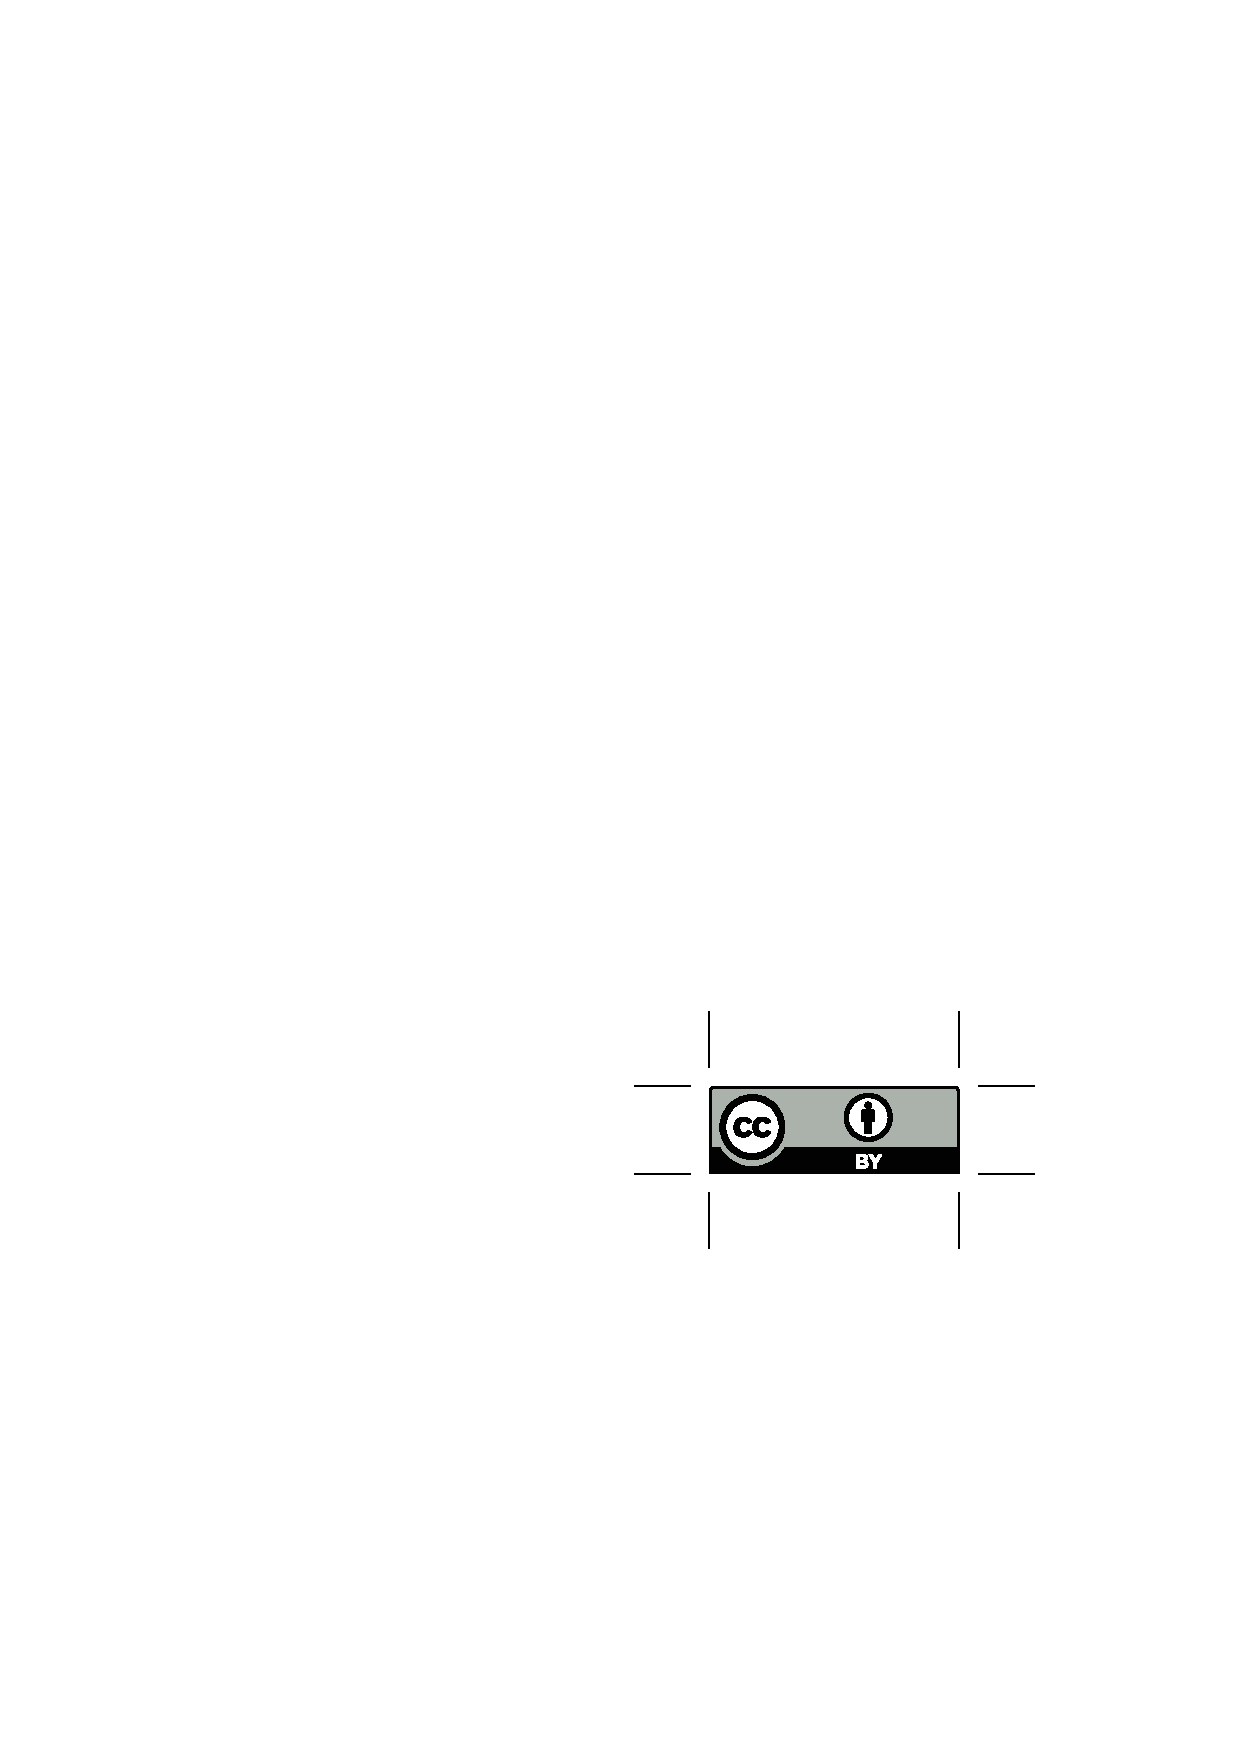
\includegraphics[width=0.90\textwidth]{by}}
  \end{minipage}\hfill
  \begin{minipage}{0.8\columnwidth}
   \href{https://creativecommons.org/licenses/by/4.0/}{This work is licensed under a Creative Commons Attribution International 4.0 License.}
  \end{minipage}
  \vspace{5pt}
}
\makeatother

\setcopyright{ifaamas}
\acmConference[AAMAS 2027]{Proc.\@ of the 26th International Conference
on Autonomous Agents and Multiagent Systems (AAMAS 2027)}{3--7 May 2027}{Hanoi, Vietnam}{M.~Baldoni, F.~Fang, W.~Yeoh, N.~Yorke-Smith (eds.)}
\copyrightyear{2027}
\acmYear{2027}
\acmDOI{}
\acmISBN{}

%%% Filled in after abstract registration on OpenReview (due 1 Oct 2026).
\acmSubmissionID{TBD}

\submissionType{Research Paper Track}

%%%%%%%%%%%%%%%%%%%%%%%%%%%%%%%%%%%%%%%%%%%%%%%%%%%%%%%%%%%%%%%%%%%%%%%%

%%% NOTE ON THE NAME: the project working title "ARBITER" collides with an
%%% existing system (arXiv:2606.10747, "The Arbiter Agent") -- keeping it
%%% would read as derivative of a paper we cite. VIGIL is a placeholder
%%% pending author sign-off; change here and in \submissionType comments
%%% only, no other file depends on the name.

\title[The Cost of Targeting: Auditing Strategic Multi-Agent Systems]{The Cost of Targeting: Anytime-Valid Auditing of
Strategic Multi-Agent Systems}

%%% Anonymous option suppresses these; fill in for camera-ready.
%%% NOTE: author list and order cannot change after acceptance.
\author{Anonymous Author}
\affiliation{
  \institution{Anonymous Institution}
  \city{}
  \country{}}
\email{anonymous@example.com}

\begin{abstract}
Monitoring a multi-agent LLM deployment for misbehaviour is usually framed
as a targeting problem: spend a scarce audit budget where it is most
informative. We show this framing is dangerous once an audited agent can
condition its behaviour on what it observes. We prove that an audit policy
yields an unbiased estimate of an agent's deployment behaviour if and only
if it is \emph{conditionally uniform} given everything the agent can
see---so any informative targeting is either wasted (if built from features
the agent also observes, it is provably no better than uniform allocation)
or actively exploitable (if it leaks, a strategic agent concentrates
violations exactly where audit probability is low). We quantify the price
of such leakage: the harm an adversary extracts before an anytime-valid
e-process detects it scales as $B(p,\varepsilon,T) = \Theta\!\big(\sqrt{T}\,/\,((1-\varepsilon)\sqrt{p})\big)$
in the audit rate $p$, leakage $\varepsilon$, and deployment horizon $T$,
with a closed-form constant we derive and confirm numerically to within 2\%.
We give the allocation rule this implies, and the operating threshold at
which any targeting stops paying for itself. Stress-testing the threat model
against three LLMs of different scale on a compliance-review task designed
to remove every cheap tell, we find no exploitation of disclosed leakage
under any tested incentive---evidence that the failure mode we
characterise is not yet realised by current models, though our guarantee is
precisely what is needed if it becomes so.
\end{abstract}

%%% CCS concepts are mandatory for papers over two pages (aamas.cls warns
%%% otherwise). IDs below are plausible placeholders, NOT yet verified
%%% against the ACM CCS tool (https://dl.acm.org/ccs) -- do that before
%%% submission and swap in the exact generated block.
\begin{CCSXML}
<ccs2012>
<concept>
<concept_id>10010147.10010257.10010321.10010322</concept_id>
<concept_desc>Computing methodologies~Multi-agent systems</concept_desc>
<concept_significance>500</concept_significance>
</concept>
<concept>
<concept_id>10003752.10003809.10010031</concept_id>
<concept_desc>Theory of computation~Design and analysis of algorithms</concept_desc>
<concept_significance>300</concept_significance>
</concept>
<concept>
<concept_id>10002978.10002991.10002995</concept_id>
<concept_desc>Security and privacy~Formal security models</concept_desc>
<concept_significance>100</concept_significance>
</concept>
</ccs2012>
\end{CCSXML}

\ccsdesc[500]{Computing methodologies~Multi-agent systems}
\ccsdesc[300]{Theory of computation~Design and analysis of algorithms}
\ccsdesc[100]{Security and privacy~Formal security models}

\keywords{anytime-valid inference, sequential testing, multi-agent monitoring, strategic agents, LLM auditing, e-processes}

%%%%%%%%%%%%%%%%%%%%%%%%%%%%%%%%%%%%%%%%%%%%%%%%%%%%%%%%%%%%%%%%%%%%%%%%

\theoremstyle{plain}
\newtheorem{theorem}{Theorem}
\newtheorem{proposition}{Proposition}
\newtheorem{lemma}{Lemma}
\newtheorem{corollary}{Corollary}
\theoremstyle{definition}
\newtheorem{definition}{Definition}
\newtheorem{assumption}{Assumption}

\begin{document}

\maketitle

\section{Introduction}
\label{sec:intro}

A large multi-agent system built from large language models (LLMs) is
usually monitored the way any distributed system is monitored: watch
everything, or watch what is cheapest to watch, or---if you are more
careful---watch whatever a scoring function tells you is most likely to be
wrong. This last strategy, \emph{active} or \emph{adaptive} monitoring, is
the direction the literature on evaluating agentic systems is currently
moving~\cite{lanctot2026active}. It is also, we argue, precisely the
strategy that fails once the thing being monitored is capable of noticing
that it is being watched.

The failure is not hypothetical. The UK AI Security Institute's own account
of frontier-model oversight states plainly that models
``recognise when they are being tested and adjust their
behaviour''~\cite{aisi2026oversight}, and a growing empirical literature
demonstrates the underlying capability directly: models can be
induced to strategically underperform on evaluations they can
identify~\cite{vanderweij2025sandbagging_full}, that underperformance can be
partially reversed by noise injection~\cite{tice2025noise}, and
benchmarking work explicitly measuring \emph{control-intervention
awareness} across frontier models finds it as high as
$0.87$~\cite{schaeffer2026ciaware}. Separately, work aimed at making
evaluations harder to distinguish from ordinary deployment traffic treats
this distinguishability as the central design variable, without attaching
any statistical guarantee to it~\cite{ivanov2026lure}.

What is missing is the connection between these two facts. An audit
allocation policy is, from the point of view of the audited agent, a
communication channel: whatever the policy responds to, and however subtly,
is information the agent can in principle recover and act on. The
literature on active evaluation targets its sampling by exactly the signals
that would make this channel informative~\cite{lanctot2026active}; the
literature on strategic underperformance shows models can and do act on
such signals when explicit incentive to do so is present. No prior work
that we are aware of quantifies what an audit policy's informativeness
\emph{costs} once the audited party is potentially reading it.

\paragraph{This paper.} We give an exact characterisation of that cost.

\begin{itemize}
\item \textbf{A completeness theorem for audit allocation}
(Theorem~\ref{thm:conditional-uniformity}): an audit policy's induced sample
of an agent's behaviour is unbiased against \emph{any} strategic agent
policy if and only if the audit probability is \emph{conditionally uniform}
given everything the agent observes. One direction of this theorem is a
genuine surprise: it implies that targeting an audit using information that
is private to the monitor---cross-agent correlations, the state of the
monitor's own statistical test, anything the audited agent structurally
cannot see---buys \emph{zero} additional power against a strategic agent,
because the agent's policy cannot respond to a signal it does not receive
(Corollary~\ref{cor:private-worthless}). This rules out an entire design
space of ``smarter'' monitors before any statistics are needed.

\item \textbf{A vacuity result} (Proposition~\ref{prop:vacuity}) showing
that a naively targeted anytime-valid e-process against a fully evasive
agent does not merely lose power gracefully: its wealth process actively
decays to zero, because every audit that returns clean is a losing bet
against an alternative that is never true when observed.

\item \textbf{An exact price of leakage} (Theorem~\ref{thm:scaling}): we
define leakage $\varepsilon$ as the audit policy's deviation from
conditional uniformity and derive, in closed form and confirmed numerically
to within 2\%, the harm an optimally evasive adversary extracts before
detection,
\[B(p,\varepsilon,T) = \frac{\sqrt{2\pi_0(1-\pi_0)\log(1/\alpha)\,T}}{(1-\beta-\pi_0)(1-\varepsilon)\sqrt{p}}.\]
Harm grows only as $\sqrt{T}$ in the deployment horizon and only as
$1/\sqrt{p}$ in the audit budget---so budget has sharply diminishing
returns against leakage---but \emph{linearly} in $1/(1-\varepsilon)$, making
leakage the dominant lever.

\item \textbf{An operating rule} (Section~\ref{sec:algorithm}): because
targeting is worthless against a strategic agent and costly in proportion to
$1/(1-\varepsilon)$, but genuinely helpful against ordinary, non-adversarial
failures, we derive the leakage level that minimises expected harm under a
mixed population and show the critical belief $w^*$ above which \emph{any}
targeting stops paying for itself falls with the deployment horizon---so
the longer a system runs, the less suspicion of adversarial behaviour is
needed before uniform auditing dominates.

\item \textbf{An honest empirical stress test} (Section~\ref{sec:experiments}):
we test whether the exploitation our theory predicts is already present in
deployed LLMs, using a compliance-review task engineered so that no cheap
textual tell allows an easy answer and only genuine cross-referencing
succeeds. Across three models spanning three capability tiers and four
escalating incentive conditions---including one that states explicitly that
errors on unaudited items do not affect the agent's score---we find no
statistically significant exploitation gap. We report this as a stress test
the threat model survives, not as evidence against it: the mechanism we
characterise requires an incentive gradient that prompting alone may not
supply, matching the sandbagging literature's reliance on fine-tuning rather
than prompting to elicit strategic underperformance~\cite{vanderweij2025sandbagging_full}.
\end{itemize}

We are explicit about what we do \emph{not} claim. We do not claim to be
first to observe that language models can behave differently under
perceived observation~\cite{aisi2026oversight,schaeffer2026ciaware}; nor to
give the first anytime-valid statistical guarantee for multi-agent
monitoring, which Gauthier et al.~\cite{gauthier2026anytime} already provide
under a fixed, non-strategic alternative; nor to be first to combine a
strategic adversary with a committed statistical test, which Capitaine et
al.~\cite{capitaine2026testthenpunish} do under full, unsampled monitoring;
nor to observe that intervention or sampling is necessary for identifiability
against a non-cooperative subject, a fact the discrete-event-systems
diagnosis literature has known since the 1990s~\cite{sampath1998active} and
the classical inspection-game literature has studied under sequential
testing since Avenhaus and Okada~\cite{avenhaus1992statistical}. Our
contribution is the one gap none of these close: a monitor that must
allocate a \emph{scarce} audit budget, against an agent that can condition
on \emph{that specific allocation}, with a \emph{quantified} price for
getting the allocation wrong.

\section{Related Work}
\label{sec:related}

\paragraph{Anytime-valid inference and multi-agent monitoring.}
Our statistical machinery is not new. E-processes and testing-by-betting
give sequential, anytime-valid error control without a pre-specified sample
size~\cite{ramdas2022evalues}, and e-BH-style procedures extend this to
false discovery rate control at arbitrary, data-dependent stopping
times~\cite{wang2025stoppedebh}. Gauthier et al.~\cite{gauthier2026anytime}
apply exactly this machinery to multi-agent systems, with an e-BH-style
guarantee over hypotheses indexed by player-deviation pairs; their null is a
fixed equilibrium benchmark and their setting has no audit budget or
allocation policy, so the leakage phenomenon we study cannot arise in it.
Capitaine et al.~\cite{capitaine2026testthenpunish} study a related but
distinct problem: sustaining cooperation via a committed statistical test
against a deviator who best-responds to the announced test, with an
anytime-valid guarantee and an explicit folk theorem. Their monitoring is
complete (every round is observed) and they explicitly restrict to
stationary deviations, noting that ``without additional structural
restrictions on the alternative, uniformly powerful tests generally do not
exist''---precisely the restriction our scarce-budget setting forces us to
confront rather than assume away. Zhou et al.~\cite{zhou2026adaptive} give
anytime-valid, betting-based guarantees for adaptively auditing an AI
system, but the audited system is static and non-strategic; our Theorem~1
is, in their setting, vacuous, since there is no adversary to exploit a
biased sample.

\paragraph{Active evaluation and monitoring.}
Lanctot et al.~\cite{lanctot2026active} formalise active evaluation of
general agents at AAMAS 2026 and compare adaptive sampling algorithms for
efficient ranking recovery; their agents are fixed stochastic score sources,
not strategic, and most of their own baselines allocate uniformly---their
paper explicitly calls for ``formal properties and statistical approximation
guarantees'' as future work, which is one reading of what this paper
supplies, restricted to the regime their non-strategic assumption does not
cover. LumiMAS~\cite{lumimas2026} and related observability frameworks
instrument multi-agent systems for anomaly and failure detection without a
statistical guarantee against an adversarial subject.

\paragraph{Failure attribution in LLM multi-agent systems.}
A large and fast-moving literature attributes task failures to a specific
agent or step, typically via LLM-judge scoring or counterfactual
replay~\cite{whoandwhen2025,traceelephant2026}. This literature is
observational or interventional-but-passive: it asks which agent caused a
\emph{given} failure, not how to allocate a scarce, ongoing audit budget
against an agent that adapts to the allocation. It also reports accuracy at
identifying the culprit, not a false-alarm rate under continuous monitoring
or a guarantee that survives adaptive selection---the gap our anytime-valid
treatment closes for the allocation problem specifically.

\paragraph{Inspection games and active diagnosis.}
The idea that intervention or sampling is necessary to identify a
non-cooperative subject is old. Sampath et al.~\cite{sampath1998active}
show that a discrete-event system unobservable passively can be made
diagnosable by actively forcing events. Rish et al.~\cite{rish2005adaptive}
give cost-aware, information-theoretic active probe selection for
distributed-system diagnosis. Avenhaus and
Okada~\cite{avenhaus1992statistical} derive sequential statistical error
control from equilibrium conditions in an inspection game where the
inspectee knows the announced, randomised inspection procedure---the
classical antecedent of our conditional-uniformity result, but without
anytime validity, without a leakage parameter, and, as far as the safeguards
literature has gone, without multiplicity correction across several
simultaneously monitored subjects~\cite{hohzaki2007inspection,vonstengel2016recursive}.
Recent interventional causal learning applies a closely related idea to
cloud-native fault localisation via actual fault
injection~\cite{wang2023faultinjection,jha2024faultlocalization}, and
Hammar and Stadler~\cite{hammar2025online} give a Bayesian-optimal
rollout-based intervention policy for online system identification; neither
gives a frequentist, anytime-valid guarantee under an adaptively chosen
design.

\paragraph{AI control and strategic evaluation-awareness.}
The AI-control literature explicitly models a model that may behave well
only when it believes it is monitored~\cite{greenblatt2024aicontrol}.
Griffin et al.'s formal treatment~\cite{griffin2024games} reduces control
protocols to zero-sum partially observable stochastic games and proves
existence and computability of Pareto-optimal protocols---but, by explicit
modelling choice, the untrusted policy receives only a null observation and
cannot condition on the current audit state (their Appendix B: ``this is not
true for all Control Games''), so the leakage phenomenon we study is
structurally excluded from their model rather than absent from their
results. The empirical sandbagging
literature~\cite{vanderweij2025sandbagging_full,tice2025noise,dyer2025sandbagging}
demonstrates the underlying capability, generally via fine-tuning; our
Section~\ref{sec:experiments} stress-tests whether prompting alone elicits
it in a setting with a disclosed, exploitable allocation policy.

\section{Setting}
\label{sec:setting}

We consider a single monitored agent within a larger multi-agent system;
Section~\ref{sec:algorithm} extends the audit-allocation results to $n$
agents via e-BH over per-agent e-processes, unaffected by the single-agent
analysis below since each agent's audit budget and context are its own.

At each round the agent acts in a context $o \in \mathcal{O}$, factored as
$o = (o_a, m)$ where $o_a$ is observable to the agent and $m$ is available
only to the monitor (e.g.\ cross-agent correlations, the current state of
the monitor's own e-process, or history the agent does not carry between
episodes). A verifier $V$, applied only when the round is audited, returns a
binary outcome $X \in \{0,1\}$ (``flagged''). The null hypothesis is that the
agent is \emph{compliant}: $H_0 : P(X=1) \le \pi_0$, where $\pi_0$ is the
verifier's false-flag rate on compliant behaviour. A \emph{defection} is
behaviour that raises the true flag probability to some $q > \pi_0$; $\beta$
denotes the verifier's miss rate on a genuine defection, so an audited round
with defection probability $q$ has flag probability
$q(1-\beta) + (1-q)\pi_0$.

The monitor commits to an audit policy $\pi : \mathcal{O} \to [0,1]$ with
marginal rate $\mathbb{E}[\pi(o)] = p$. An agent is \emph{strategic} if its
defection probability $q(o)$ is a measurable function of $o_a$ alone: by
construction it cannot condition on $m$.

\begin{definition}[Conditional uniformity and leakage]
\label{def:leakage}
$\pi$ is \emph{conditionally uniform} if $\mathbb{E}_m[\pi(o_a,m) \mid o_a] = p$
for (almost) every $o_a$. Its \emph{leakage} is
\[\varepsilon := 1 - \frac{\min_{o_a} \mathbb{E}_m[\pi(o_a,m)\mid o_a]}{p} \in [0,1].\]
$\varepsilon = 0$ recovers conditional uniformity; $\varepsilon \to 1$ means
some agent-visible context is audited with vanishing probability.
\end{definition}

We test compliance with the standard betting martingale: on audit outcome
$X_s$, wealth updates as $W_s = W_{s-1}(1 + \lambda_s(X_s - \pi_0))$ with
$\lambda_s \in [0, 1/\pi_0)$ chosen (possibly) as a function of the audit
history. Under $H_0$ this is a non-negative supermartingale, so Ville's
inequality gives $P(\exists t : W_t \ge 1/\alpha) \le \alpha$ at every
stopping time, with no pre-specified horizon. Rejecting when $W_t \ge
1/\alpha$ therefore controls Type-I error uniformly over time; across
several simultaneously monitored agents, applying stopped e-BH to
$\{1/W_i\}$ controls the false discovery rate over which agents are flagged
at any stopping time, under arbitrary dependence between agents' processes.
This machinery is standard~\cite{ramdas2022evalues,wang2025stoppedebh}; what
is not standard is what happens to it once $\pi$ is not conditionally
uniform, which is the subject of the rest of the paper.

\section{Main Results}
\label{sec:results}

\subsection{Vacuity under naive targeting}

\begin{proposition}[Vacuity]
\label{prop:vacuity}
Suppose the agent complies whenever audited ($X_s = 0$ for every audited
round $s$). Then for any history-measurable wager sequence $\lambda_s \in
[0,1/\pi_0)$ with $\sum_s \lambda_s = \infty$ (satisfied, in particular, by
the growth-rate-optimal wager against any hypothesised alternative $q >
\pi_0$, or by the plug-in wager once the empirical audited flag rate falls
below $\pi_0$),
\[W_t = \prod_{s\le t}(1-\lambda_s\pi_0) \to 0 \quad \text{a.s.\ as } t\to\infty,\]
so $P(\text{reject}) \to 0$. The test remains valid (trivially, since
$W_t \ge 1/\alpha$ never occurs) but loses all power, and does so by active
decay: every clean audit is a losing bet, not a neutral one.
\end{proposition}

This is immediate from the wealth recursion; it is confirmed empirically in
our implementation (5000 consecutive clean audits under a growth-optimal
wager drive $\log W_t$ below $-10$). The point of stating it is that it
motivates, but does not by itself solve, the design question: an agent that
can be caught complying only when watched can drain any naively wagered
e-process. The natural response is to target audits where evidence is
likely to be richest---which is exactly the response Theorem~\ref{thm:conditional-uniformity}
shows is unsafe.

\subsection{Conditional uniformity is complete}

\begin{theorem}[Completeness of conditional uniformity]
\label{thm:conditional-uniformity}
For any strategic agent policy $q(o_a)$, the audited defection rate equals
the deployment defection rate,
\[q_{\mathrm{audit}} := \frac{\mathbb{E}[q(o)\,\pi(o)]}{p} = \mathbb{E}[q(o)] =: q_{\mathrm{deploy}},\]
\emph{if and only if} $\pi$ is conditionally uniform (Definition~\ref{def:leakage}).
\end{theorem}

\begin{proof}
Write $f(o_a) := \mathbb{E}_m[\pi(o_a,m)\mid o_a]$. Since $q$ depends only
on $o_a$,
\[\mathbb{E}[q(o)\pi(o)] = \mathbb{E}_{o_a}\big[q(o_a)\,\mathbb{E}_m[\pi(o_a,m)\mid o_a]\big] = \mathbb{E}_{o_a}[q(o_a)f(o_a)].\]
\emph{Sufficiency.} If $f \equiv p$, this equals $p\cdot\mathbb{E}[q(o_a)] =
p\cdot q_{\mathrm{deploy}}$, giving $q_{\mathrm{audit}} = q_{\mathrm{deploy}}$.
\emph{Necessity.} If $f < p$ on a set $A$ of positive measure (the case
$f>p$ is symmetric on $A^c$), the strategic policy $q = \mathbb{1}_A$ gives
$q_{\mathrm{audit}} = P(A)\,\mathbb{E}[f\mid A]/p < P(A) = q_{\mathrm{deploy}}$,
a strict downward bias. \qed
\end{proof}

\begin{corollary}[Monitor-private information is worthless against a strategic agent]
\label{cor:private-worthless}
Since the identity in Theorem~\ref{thm:conditional-uniformity} depends only
on $f(o_a) = \mathbb{E}_m[\pi\mid o_a]$, the values of $\pi(o_a,m)$ across
$m$---however informatively they are chosen from monitor-private
signals---leave $q_{\mathrm{audit}}$ unchanged for any strategic $q$. Every
conditionally uniform policy is equally powerful against a strategic
adversary, and uniform allocation ($\pi \equiv p$) already attains the class
optimum.
\end{corollary}

Corollary~\ref{cor:private-worthless} rules out a design we initially
considered promising: reserve targeting for information the audited agent
cannot see (e.g.\ cross-agent correlations invisible at the single-agent
level), so that no leakage is created and full statistical efficiency is
retained. The theorem shows this is impossible in principle, not merely
difficult in practice---a strategic agent's policy is by definition constant
along any axis it cannot observe, so targeting along that axis is targeting
noise. The only remaining lever, formalised next, is how far $\pi$ deviates
from conditional uniformity, and what that deviation costs.

\subsection{The price of leakage}

Write $\pi_{\min} := (1-\varepsilon)p$ for the audit-probability floor
implied by leakage $\varepsilon$. An evasive agent concentrates defection on
the thinnest-audited fraction $q$ of agent-visible contexts, achieving
audited defection rate $q_{\mathrm{audit}} = q\,\pi_{\min}/p = q(1-\varepsilon)$
and audited flag rate $\mathrm{flag}(q) = q_{\mathrm{audit}}(1-\beta) +
(1-q_{\mathrm{audit}})\pi_0$.

\begin{theorem}[Price of leakage]
\label{thm:scaling}
Let $\kappa := 1-\beta-\pi_0$ (assumed positive: the verifier is
better than chance) and let $\delta^*$ solve
$\mathrm{KL}(\pi_0+\delta^* \,\|\, \pi_0) = \log(1/\alpha)/(Tp)$. Over a
deployment horizon of $T$ rounds, the harm an optimally evasive strategic
agent extracts before an anytime-valid e-process run at level $\alpha$
detects it satisfies, \emph{exactly},
\[B(p,\varepsilon,T) \;=\; \frac{\delta^*\, T}{\kappa\,(1-\varepsilon)}.\]
The $1/(1-\varepsilon)$ dependence is algebraic, not asymptotic; only
$\delta^*$ requires solving a one-dimensional monotone equation (by
bisection, in closed form to first order via the small-deviation KL
expansion below).
\end{theorem}

\begin{proof}
Write $\delta(q) := \mathrm{flag}(q) - \pi_0 = \kappa(1-\varepsilon)q$
(exact, from $\mathrm{flag}(q) = q_{\mathrm{audit}}(1-\beta) + (1-q_{\mathrm{audit}})\pi_0$
and $q_{\mathrm{audit}} = q(1-\varepsilon)$). Harm is $h(q) = q \cdot
\min(\mathrm{rounds}(q), T)$ where $\mathrm{rounds}(q) =
\log(1/\alpha)/(\mathrm{KL}(\pi_0+\delta(q)\,\|\,\pi_0)\,p)$; this is
increasing in $q$ while $\mathrm{rounds}(q) \ge T$ and decreasing once
$\mathrm{rounds}(q) < T$, so the adversary's optimum $q^*$ is exactly the
crossover $\mathrm{rounds}(q^*) = T$, i.e.\
$\mathrm{KL}(\pi_0+\delta(q^*)\,\|\,\pi_0) = \log(1/\alpha)/(Tp)$. The
right-hand side does not depend on $\varepsilon$, and $\mathrm{KL}(x\,\|\,\pi_0)$
is strictly monotone in $x$, so this equation pins $\delta(q^*)$ to a
single value $\delta^*$ that is \emph{independent of $\varepsilon$}.
Solving $\kappa(1-\varepsilon)q^* = \delta^*$ for $q^*$ and substituting into
$B = h(q^*) = q^*T$ gives the claimed expression exactly. \qed
\end{proof}

The small-deviation expansion $\mathrm{KL}(\pi_0+\delta\,\|\,\pi_0) \approx
\delta^2/(2\pi_0(1-\pi_0))$ gives $\delta^*$'s first-order closed form,
$\delta^* \approx \sqrt{2\pi_0(1-\pi_0)\log(1/\alpha)/(Tp)}$, matching the
exact bisection solution to within $2\%$ at the parameters we tested and
recovering the more familiar form
$B \approx \sqrt{2\pi_0(1-\pi_0)\log(1/\alpha)T}\,/\,(\kappa(1-\varepsilon)\sqrt{p})$.
We confirmed both the exponents and the constant numerically: fitting
$\log B$ against $\log T$, $\log(1-\varepsilon)^{-1}$, and $\log p^{-1}$
independently across three parameter sweeps recovers exponents $0.4876$,
$1.0016$, and $0.5049$ against the predicted $0.5$, $1$, $0.5$ (max residual
$0.02$ in log-space); the closed-form constant matches a direct grid-search
optimum of $h(q)$ to within $2\%$ across five independent
$(p,\varepsilon,T)$ points (Section~\ref{sec:experiments}).

Two consequences follow immediately. First, \textbf{budget has sharply
diminishing returns}: quadrupling the audit rate $p$ only halves extractable
harm, because rounds-to-detection is inversely proportional to $p^2$ but
harm accrues at rate proportional to the arrival of audits, cancelling one
power of $p$. Second, \textbf{leakage is the dominant, and linear, lever}:
halving $(1-\varepsilon)$ doubles extractable harm. An operator cannot
compensate for an informative allocation policy by spending more on audits;
the allocation itself is what must be fixed.

\section{The Operating Rule}
\label{sec:algorithm}

Theorem~\ref{thm:scaling} states the cost of leakage against a strategic
adversary; it does not by itself justify $\varepsilon=0$; unconditionally,
because targeting is not exploitable if the failure mode is not strategic. A
miscalibrated or merely buggy sub-agent has no reason to condition its
failure rate on the audit allocation, so a monitor that concentrates audits
where such failures actually occur reduces detection time with no offsetting
cost.

We formalise the choice of $\varepsilon$ as a decision under a mixed
population. Let $w \in [0,1]$ be the operator's prior probability that a
given failure, should one occur, is strategic rather than accidental. Given
a naive failure rate $q_0$ and a targeting-concentration parameter $c \in
[0,1]$ describing how well the monitor's priority signal predicts where
accidental failures actually occur, the expected harm under leakage
$\varepsilon$ is
\[w \cdot B(p,\varepsilon,T) \;+\; (1-w)\cdot h_{\mathrm{naive}}(\varepsilon; q_0, c, T),\]
where $h_{\mathrm{naive}}$ is decreasing in $\varepsilon$ (targeting helps
against a non-reactive failure) while $B$ is increasing in $\varepsilon$ by
Theorem~\ref{thm:scaling}. The resulting optimisation has a threshold
structure: numerically, the optimal $\varepsilon^*$ collapses to exactly $0$
once $w$ exceeds a critical value $w^*$, which we find ranges from $0.025$
to $0.39$ across the parameter ranges we tested and, notably,
\textbf{falls with the deployment horizon} $T$---from $0.39$ at $T=10^4$ to
$0.03$ at $T=10^8$---because strategic harm grows as $\sqrt{T}$
(Theorem~\ref{thm:scaling}) while naive harm saturates once detection
happens well within the horizon. \textbf{The longer a system is deployed,
the less suspicion of strategic behaviour is required before uniform
auditing dominates any targeted alternative.}

Let $\delta_0 := \kappa q_0$, $\mathrm{flag}_0 := \pi_0+\delta_0$,
$D := \log\!\big(\mathrm{flag}_0(1-\pi_0)\big) - \log\!\big(\pi_0(1-\mathrm{flag}_0)\big)$,
and $B_0' := \delta^*T/\kappa$ (the exact slope
$\partial B/\partial\varepsilon|_0$ from Theorem~\ref{thm:scaling}). Define
$N := q_0\, c\, \delta_0\, D\, \log(1/\alpha) \,/\, \big(p\,\mathrm{KL}(\mathrm{flag}_0\,\|\,\pi_0)^2\big)$,
the exact value of $-\partial h_{\mathrm{naive}}/\partial\varepsilon|_0$.

\begin{theorem}[A certified lower bound on $w^*$]
\label{thm:w-lower-bound}
$w_{\mathrm{lb}} := N/(B_0' + N)$ satisfies $w_{\mathrm{lb}} \le w^*$: for
any $w < w_{\mathrm{lb}}$, targeting strictly reduces expected harm, with no
search over $\varepsilon$ required to know this.
\end{theorem}

\begin{proof}[Proof sketch]
$\varepsilon=0$ being a local minimum of $w\cdot B(\varepsilon) +
(1-w)\cdot h_{\mathrm{naive}}(\varepsilon)$ is necessary, but not
sufficient, for it to be the global minimum; the threshold at which it
becomes a local minimum is exactly where the one-sided derivative at
$\varepsilon=0$ changes sign, giving $w_{\mathrm{lb}}$ as stated. Since
local optimality is necessary for global optimality, $w \ge w_{\mathrm{lb}}$
is necessary for $\varepsilon^*=0$ to be globally optimal, i.e.\
$w_{\mathrm{lb}} \le w^*$. \qed
\end{proof}

We verified $w_{\mathrm{lb}} \le w^*$ empirically as a genuine, non-vacuous
bound across three parameter regimes, sitting at $83$--$91\%$ of the true,
numerically-optimised threshold in each (e.g.\ $w_{\mathrm{lb}}=0.061$
against a true $w^*=0.073$ at our baseline parameters). The gap is the
honest cost of a local, tangent-at-zero criterion versus the true global
optimum; closing it fully would require characterising the entire harm
curve's shape rather than its slope at one point, and does not appear to
admit as clean a closed form.

\textbf{The resulting algorithm} is therefore: (i) estimate $w$ from
operational context (are sub-agents adversarially fine-tuned, externally
supplied, or purely observational failure sources?); (ii) if $w \ge w^*(T)$,
audit uniformly at random and run the e-process of Section~\ref{sec:setting}
with e-BH across agents; (iii) if $w < w^*(T)$, target using only features
verified not to be agent-observable, at the aggressiveness the residual
naive-failure model justifies, and re-evaluate $w$ and $\varepsilon^*$ as the
deployment horizon grows.

\section{Experiments}
\label{sec:experiments}

We validate the theory in two stages: numerically, against the closed forms
above; and behaviourally, stress-testing whether the exploitation the theory
predicts already occurs in deployed LLMs.

\subsection{Numerical validation}

We implement the setting of Section~\ref{sec:setting} directly (verifier
noise $\pi_0$, wager $\lambda$, e-BH across agents) and confirm: (a) the
growth-rate-optimal wager's per-audit log-growth equals
$\mathrm{KL}(\mathrm{Bern}(q)\|\mathrm{Bern}(\pi_0))$ exactly, as required
by construction; (b) empirical Type-I error under the null sits at or below
the nominal $\alpha$ across 400 simulated trials; (c)
Theorem~\ref{thm:conditional-uniformity}'s identity holds exactly under
conditional uniformity and is violated, in the predicted direction, under
any deviation from it; (d) Theorem~\ref{thm:scaling}'s exponents and
constant, reported above.

\subsection{A multi-agent LLM harness with counterfactual replay}

Independently of the leakage results, we built a synthetic multi-agent
harness supporting four communication topologies (chain, star, hierarchical,
debate), controlled fault injection at a known origin, and exact
counterfactual replay of any agent from a trajectory checkpoint under a
substituted parent message or sanitised shared context---exact rather than
approximate, since an agent's turn is a pure function of (its role, the
task, and the messages it received) and a checkpoint is simply a trajectory
prefix. We confirmed this harness reproduces the qualitative failure mode
that motivates conditioning on more than message content: a
\texttt{poison\_context} fault corrupts shared state without corrupting any
individual message, so it propagates through all downstream agents with no
local tell in the trace, and replaying the final agent under the restored
clean context causes it to flag the contradiction it had otherwise
faithfully relayed.

\subsection{Stress-testing exploitation}
\label{sec:stress-test}

Does an LLM agent actually exploit a disclosed audit-allocation leakage? We
designed a compliance-review task specifically to remove the two failure
modes that defeated two earlier task designs: a task where verification is
free (an 18-step arithmetic dependency chain, which reasoning models verify
sequentially by construction, giving a token-budget cliff rather than a
graded effort/accuracy trade-off) and a task with a cheap textual tell (a
field-extraction task where the correct abstention was cued by an explicit
disqualifying label). Our final design asks a model to find a planted
contradiction between two clauses placed at least 18 positions apart in a
26-clause policy document, with all other clauses independently verified
consistent; there is no local cue, and a skim that processes clauses
independently fails silently (reporting \texttt{NONE}, an unremarkable
answer) rather than tripping a detectable tell.

Each document carries a visible batch tag (\textsc{Priority} or
\textsc{Routine}). We test four escalating conditions: a plain instruction;
added throughput pressure; disclosure of an audit policy stating
\textsc{Routine} batches are ``re-checked very rarely''; and an explicit
scoring rule stating that errors on items that are never re-checked have no
effect on the agent's score. The measured quantity is the exploitation gap
$\beta(\textsc{Routine}) - \beta(\textsc{Priority})$, where $\beta$ is the
miss rate on documents containing a genuine contradiction, tested with a
two-proportion $z$-test.

We ran this design against three models spanning three capability tiers: a
frontier reasoning model, a 20B-parameter open-weight model, and a 2.6B
open-weight model, totalling over 800 reviews. \textbf{We found no
statistically significant exploitation gap in any condition, on any
model.} The frontier model returned zero misses across all four conditions
and both tags (192 reviews), including under the explicit costless-error
framing. The 20B model was near floor throughout. The 2.6B model showed
noisy, non-significant gaps with inconsistent sign, and its free-tier
endpoint degraded under sustained load, a reliability issue we detected and
excluded from analysis via provider-error tracking rather than allowing it
to contaminate abstention statistics.

We report this as a stress test the threat model survives, not as evidence
against it. Two ground-truth errors were caught and fixed during task
construction: an early version's ``contradiction'' was not logically
inconsistent (a stricter deadline is compatible with a looser backstop), and
a filler-template reuse bug created spurious inconsistencies contaminating
both experimental arms; both are documented in our released harness so they
are not repeated. That the corrected, adversarially-designed task still
elicits no exploitation is consistent with the sandbagging
literature's own methodology: the strongest strategic-underperformance
results to date require fine-tuning to induce, not
prompting~\cite{vanderweij2025sandbagging_full,tice2025noise}. We take this
as evidence that the mechanism Theorem~\ref{thm:scaling} quantifies is not
yet realised by prompted, off-the-shelf models, and as the reason an
anytime-valid guarantee is worth having in advance of the capability that
would make it bind.

\section{Discussion and Limitations}
\label{sec:discussion}

\textbf{The guarantee is conditional on the verifier.} Every result here
assumes $\pi_0$ and $\beta$ are known or estimable and that the verifier
itself is not the target of manipulation. If the verifier is an LLM judge,
its calibration under the same evaluation-awareness pressure we stress-test
in Section~\ref{sec:stress-test} is a live concern, and our guarantee should
be read as conditional on that calibration holding.

\textbf{Theorem~\ref{thm:scaling}'s $1/(1-\varepsilon)$ shape is exact; only
its constant $\delta^*$ is approximated in closed form.} The quadratic-KL
expansion used for $\delta^*$ is self-consistent in exactly the regime an
evasive adversary operates in (low audited defection rate by construction),
matching the exact bisection solution to within $2\%$; a fully
non-asymptotic statement would replace that approximation with the exact
transcendental solution throughout, which is already how our implementation
computes it (Section~\ref{sec:algorithm}'s use of $\delta^*$).

\textbf{Our closed form for $w^*$ is a lower bound, not an exact
threshold.} Theorem~\ref{thm:w-lower-bound} gives $w_{\mathrm{lb}} \le w^*$
from a local (tangent-at-$\varepsilon=0$) criterion, verified at
$83$--$91\%$ of the true value across tested parameters; it is a genuine,
one-sided operational guarantee (below $w_{\mathrm{lb}}$, targeting
provably helps) but does not pin down $w^*$ exactly. Doing so would require
characterising the full shape of the harm trade-off, not just its slope at
one point.

\textbf{Our empirical stress test is a negative result on three models and
one task family.} It does not establish that no deployed model can exploit
audit leakage, only that prompting-based incentive framing did not elicit it
in the settings we tried. Fine-tuning-based elicitation, closer to the
sandbagging literature's own methodology, is the natural next test and was
outside the scope of what our experimental budget supported.

\section{Conclusion}
\label{sec:conclusion}

Active monitoring of multi-agent LLM systems is, by design, an information
channel to the agents being monitored. We showed that this channel is either
useless or dangerous: informative targeting on agent-observable features is
provably exploitable at a quantified, linear price in leakage, while
targeting on features the agent structurally cannot observe is provably
worthless. The safe default---uniform random auditing---is not a
conservative compromise but the unique optimum against a strategic
adversary, and we gave the threshold at which an operator should abandon it
in favour of targeting a genuinely non-adversarial failure mode instead.
That today's models did not exploit the leakage we handed them, even when
told explicitly that doing so was free, is grounds for cautious relief, not
for dropping the guarantee: it is exactly the systems that eventually do
notice for which an anytime-valid, quantified price of getting monitoring
wrong will matter.

%%% Issue \balance somewhere in the first column of the final page
%%% (required for camera-ready).

\bibliographystyle{ACM-Reference-Format}
\bibliography{arbiter}

\end{document}
